%------------------------------------------------------------------------------
% CV in Latex
% Author : Charles Rambo
% Based off of: https://github.com/sb2nov/resume and Jake's Resume on Overleaf
% Most recently updated version may be found at https://github.com/fizixmastr 
% License : MIT
%------------------------------------------------------------------------------

%\documentclass[A4,11pt]{article}
\documentclass[A4, 11pt, UTF8]{ctexart}
\usepackage[T1]{fontenc}
%\documentclass[letterpaper,11pt]{article} %For use in US
\usepackage{latexsym}
\usepackage[empty]{fullpage}
\usepackage{titlesec}
\usepackage{marvosym}
\usepackage[usenames,dvipsnames]{color}
\usepackage{verbatim}
\usepackage{enumitem}
\usepackage[hidelinks]{hyperref}
\usepackage[english]{babel}
\usepackage{tabularx}
\usepackage{tikz}
\input{glyphtounicode}

\begin{comment}
I am by no means a professional when it comes to the CV's/resumes, I have
received various trainings on how to write a CV and resume from my high 
school, as well as the Austin College and University of Eastern Finland's
career counseling departments. As I intend to share my CV as a template, I 
feel that it is my responsibility to provide explanations of my work.
\end{comment}


%-----FONT OPTIONS-------------------------------------------------------------
\begin{comment}
The font of the document will impact not just how readable it is, but how it is
perceived. In the "The Craft of Scientific Writing" by Michael Alley, shares a
common fonts for publication as well as their use. I have chosen to use
Palatino for its legibility, some others are given below. There is far too much
about typography to discus here. Note: serif fonts have short projecting
strokes, sans-serif fonts are sans (without) these strokes.
\end{comment}


% serif
\usepackage{palatino}
% \usepackage{times} %This is the default as well
% \usepackage{charter}

% sans-serif
% \usepackage{helvet}
% \usepackage[sfdefault]{noto-sans}
% \usepackage[default]{sourcesanspro}

%-----PAGE SETUP---------------------------------------------------------------

% Adjust margins
\addtolength{\oddsidemargin}{-1cm}
\addtolength{\evensidemargin}{-1cm}
\addtolength{\textwidth}{2cm}
\addtolength{\topmargin}{-1cm}
\addtolength{\textheight}{2cm}

% Margins for US Letter size
%\addtolength{\oddsidemargin}{-0.5in}
%\addtolength{\evensidemargin}{-0.5in}
%\addtolength{\textwidth}{1in}
%\addtolength{\topmargin}{-.5in}
%\addtolength{\textheight}{1.0in}

\urlstyle{same}

\raggedbottom
\raggedright
\setlength{\tabcolsep}{0cm}

% Sections formatting
\titleformat{\section}{
	\vspace{-4pt}\scshape\raggedright\large
}{}{0em}{}[\color{black}\titlerule \vspace{-5pt}]

% Ensure that .pdf is machine readable/ATS parsable
\pdfgentounicode=1

%-----CUSTOM COMMANDS FOR FORMATTING SECTIONS----------------------------------
\newcommand{\CVItem}[1]{
	\item\small{
		{#1 \vspace{-2pt}}
	}
}

\newcommand{\CVSubheading}[4]{
	\vspace{-2pt}\item
	\begin{tabular*}{0.97\textwidth}[t]{l@{\extracolsep{\fill}}r}
		\textbf{#1} & #2 \\
		\small#3 & \small #4 \\
	\end{tabular*}\vspace{-7pt}
}

\newcommand{\CVSubSubheading}[2]{
	\item
	\begin{tabular*}{0.97\textwidth}{l@{\extracolsep{\fill}}r}
		\text{\small#1} & \text{\small #2} \\
	\end{tabular*}\vspace{-7pt}
}

\newcommand{\CVSubItem}[1]{\CVItem{#1}\vspace{-4pt}}

\renewcommand\labelitemii{$\vcenter{\hbox{\tiny$\bullet$}}$}

\newcommand{\CVSubHeadingListStart}{\begin{itemize}[leftmargin=0.5cm, label={}]}
	% \newcommand{\resumeSubHeadingListStart}{\begin{itemize}[leftmargin=0.15in, label={}]} % Uncomment for US
		\newcommand{\CVSubHeadingListEnd}{\end{itemize}}
	\newcommand{\CVItemListStart}{\begin{itemize}}
		\newcommand{\CVItemListEnd}{\end{itemize}\vspace{-5pt}}
	
	%------------------------------------------------------------------------------
	% CV STARTS HERE  %
	%------------------------------------------------------------------------------
	\begin{document}

		
		\begin{minipage}[c]{0.05\textwidth}
			\-\
		\end{minipage}
		\begin{minipage}[c]{0.2\textwidth}
			{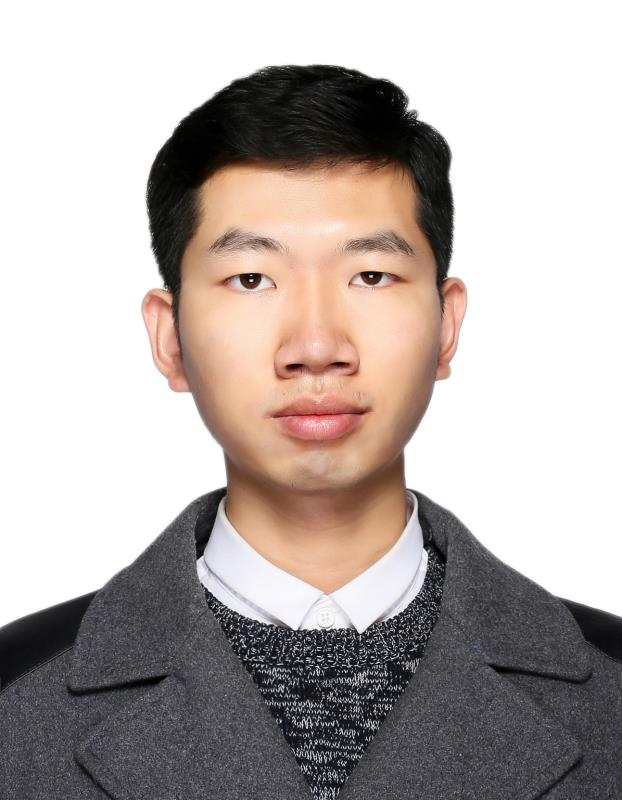
\includegraphics[width = 3cm]{photo}}
%			\begin{tikzpicture}
%				\clip (0,0) circle (1.75cm);
%				\node at (0,-.7) {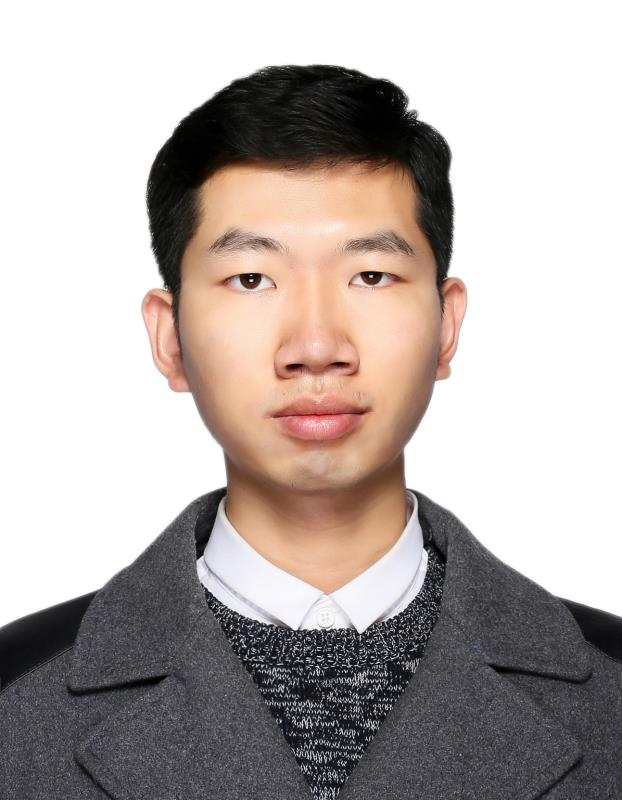
\includegraphics[width = 3cm]{photo}}; 
%				% if necessary the picture may be moved by changing the at (coordinates)
%				% width defines the 'zoom' of the picture
%			\end{tikzpicture}
			\hfill\vline\hfill
		\end{minipage}
		\begin{minipage}[c]{0.4\textwidth}
			\textbf{\Huge \scshape{郭亨}} \\ \vspace{3pt} 
			% \scshape sets small capital letters, remove if desired
			{电话:\underline{18582521993}} \\
			\href{mailto:heng.guo@ist.osaka-u.ac.jp}{邮箱:\underline{heng.guo@ist.osaka-u.ac.jp}}\\
			% Be sure to use a professional *personal* email address
			\href{https://gh-home.github.io/}{个人主页:\underline{https://gh-home.github.io}} \\
			% you should adjust you linked in profile name to be professional and recognizable
		\end{minipage}
		
		% Without picture
		%\begin{center}
			%    \textbf{\Huge \scshape Charles Rambo} \\ \vspace{1pt} %\scshape sets small capital letters, remove if desired
			%    \small +1 123-456-7890 $|$ 
			%    \href{mailto:you@provider.com}{\underline{you@provider.com}} $|$\\
			%    % Be sure to use a professional *personal* email address
			%    \href{https://linkedin.com/in/your-name-here}{\underline{linkedin.com/in/charles-rambo}} $|$
			%    % you should adjust you linked in profile name to be professional and recognizable
			%    \href{https://github.com/fizixmastr}{\underline{github.com/fizixmastr}}
			%\end{center}

	
		
		%-----EDUCATION----------------------------------------------------------------
		\section{教育经历}
		\CVSubHeadingListStart
		%    \CVSubheading % Example
		%      {Degree Achieved}{Years of Study}
		%      {Institution of Study}{Where it is located}
		\CVSubheading
		{{Master of Science $|$ \emph{\small{Photonics}}}}{Aug. 2019 -- May 2021}
		{University of Eastern Finland}{Joensuu, Finland}
		\CVSubheading
		{{Bachelor of Arts $|$ \emph{\small{Major: Physics, Minor: Education}}}}{Aug. 2016 -- May 2018}
		{Austin College}{Sherman, TX}
		\CVSubheading
		{Associate of Liberal Sciences}{Aug. 2015 -- May 2016}
		{North Lake College}{Irving, TX}
		\CVSubHeadingListEnd
		
		%-----WORK EXPERIENCE----------------------------------------------------------
		\begin{comment}
		try to briefly explain what you did and why it is relevant to the position you
		are seeking
		\end{comment}
		
		\section{Work Experience}
		\CVSubHeadingListStart
		%    \CVSubheading %Example
		%      {What you did}{When you worked there}
		%      {Who you worked for}{Where they are located}
		%      \CVItemListStart
		%        \CVItem{Why it is important to this employer}
		%      \CVItemListEnd
		\CVSubheading
		{Integration Engineering Intern}{June 2018 -- August 2019}
		{Finisar Corp.}{Sherman, TX}
		\CVItemListStart
		\CVItem{Worked in ISO 4 cleanroom developing applications to improve efficiency and creating specs}
		\CVItem{Employed metrology and microscopy for failure analysis and developing process for wet etching}
		\CVItem{Member of Emergency Response Team}
		\CVItemListEnd
		\CVSubheading
		{Laboratory Assistant}{January 2016 -- July 2016}
		{North Lake College}{Irving, TX}
		\CVItemListStart
		\CVItem{Inventoried and maintained Physics Department lab equipment}
		\CVItem{Physics tutoring}
		\CVItemListEnd
		\CVSubheading
		{Assistant Manager}{December 2006 -- August 2015}
		{Sun \& Ski Sports}{Austin, TX}
		\CVItemListStart
		\CVItem{Led a team of 20+ employees}
		\CVItem{Ran social media, as well as all grassroots marketing}
		\CVItemListEnd
		\CVSubHeadingListEnd
		
		%-----PROJECTS AND RESEARCH----------------------------------------------------
		\begin{comment}
		Ideally the title of the work should speak for what it is. However if you feel
		like you should explain more about why the project is applicable to this job,
		use item list as is shown in the work experience section.
		\end{comment}
		
		\section{Projects and Research}
		\CVSubHeadingListStart
		%    \CVSubheading
		%      {Title of Work}{When it was done}
		%      {Institution you worked with}{unused}
		\CVSubheading
		{{Surface Plasmon Propagation in the Kretschmann-Raether Configuration} $|$ \emph{\small{Python}}}{Fall 2020}
		{University of Eastern Finland}{}
		\CVSubheading
		{{Simulation of Vector Beams Through High Numerical Aperture Lens} $|$ \emph{\small{Python}}}{Fall 2020}
		{University of Eastern Finland}{}
		\CVSubheading
		{Characterization of the Flame-S Spectrometer for Spectral Imaging Research}{Spring 2020}
		{University of Eastern Finland}{}
		\CVSubheading
		{{Free Form Lens Systems for 3D Printing} $|$ \emph{\small{MATLAB, OpTaliX}}}{Spring 2019}
		{University of Eastern Finland}{}
		\CVSubheading
		{Procedures for Plating and Wet-Etching in III-V Semiconductor Devices}{Summer 2019}
		{Finisar Corp.}{}
		\CVSubheading
		{Photo-Filter Characterization for Photometric Identification of Be Stars}{Fall 2017}
		{Austin College}{}
		\CVSubheading
		{Improved Calibrating Equations for Volumetric Soil Moisture Measurement}{Spring 2017}
		{Austin College}{}
		\CVSubheading
		{{Product Design, and Manufacturing Using 3D Printing} $|$ \emph{\small{Autodesk 123D}}}{Fall 2016}
		{Austin College}{}
		\CVSubHeadingListEnd
		
			
		%-----------PROJECTS-----------
		\section{获奖荣誉}
		\resumeSubHeadingListStart
		\resumeProjectHeading
		{Meeting on Image Recognition and Understanding 最佳学生论文 (Top 1\%)}{2020年4月}
		\resumeProjectHeading
		{电子科技大学优秀毕业论文 (Top 3\%)}{2018年6月}
		\resumeProjectHeading
		{电子科技大学优秀硕士毕业生 (Top 6\%)}{2018年6月}
		\resumeProjectHeading
		{研究生国家奖学金 (Top 2\%))}{2017年10月}
		\resumeProjectHeading
		{电子科技大学学术奖学金 (Top 10\%)}{2015 \& 2016 \& 2017}
		\resumeProjectHeading
		{电子科技大学优秀毕业生 (Top 7\%)}{2015年9月}
		\resumeProjectHeading
		{全国信息安全竞赛一等奖}{2014年7月}
		\resumeProjectHeading
		{四川省电子设计竞赛二等奖}{2013年9月}
		\resumeProjectHeading
		{人民奖学金 (Top 15\%)}{2011 \& 2012 \& 2013}
		%	%   \resumeProjectHeading
		%	%   {Outstanding Individual in Social Practice}{Sep. 2012}
		\resumeSubHeadingListEnd
		
		%-----------PROJECTS-----------
		\section{发表论文}
		%\renewcommand\labelenumi{(\theenumi)}
		\begin{enumerate}[label={[\arabic*]}]
			\item Guo Heng, et al. ``Patch-based uncalibrated photometric stereo under natural illumination" 
			IEEE Transactions on Pattern Analysis and Machine Intelligence. (\textbf{TPAMI 2021}) [SCI 1区, 影响因子:16.39]. 
			\item Guo Heng, et al. ``Multispectral Photometric Stereo for Spatially-Varying Spectral Reflectances: A well posed problem?" IEEE Conference on Computer Vision and Pattern Recognition. (\textbf{CVPR 2021}) [CCF A类, H5-index:356]. 
			\item Guo Heng, et al. ``Self-calibrating Near-light Photometric Stereo under Anisotropic Light Emission." Meeting on Image Recognition and Understanding (\textbf{MIRU 2020 最佳学生论文}).  
			\item Guo Heng, et al. ``Joint video stitching and stabilization from moving cameras." IEEE Transactions on Image Processing (\textbf{TIP 2016}) [SCI 1区, 影响因子:6.79].
			\item Guo Heng, et al. ``View-consistent meshflow for stereoscopic video stabilization." IEEE Transactions on Computational Imaging (\textbf{TCI 2018}) [SCI 2区, 影响因子:3.49].
			\item Guo Heng, et al. ``Joint bundled camera paths for stereoscopic video stabilization." IEEE International Conference on Image Processing (\textbf{ICIP 2016 Oral}) [CCF C类, H5-index:60].
			\item Guo Heng, et al. ``Multispectral Photometric Stereo for Spatially-Varying Spectral Reflectances" International Journal of Computer Vision. (IJCV minor revision) [SCI 1区, 影响因子:7.41]. 
			\item Guo Heng, et al. ``Parametric Near-light Photometric Stereo" IEEE Conference on Computer Vision and Pattern Recognition. (CVPR 2022 under review). 
			\item Guo Heng, et al. ``NeuralMPS: Multispectral Photometric Stereo for Non-lambertian Spectral Reflectance" IEEE Conference on Computer Vision and Pattern Recognition. (CVPR 2022 under review). 
		\end{enumerate}
		
	\end{document}